\documentclass[main.tex]{subfiles}


\begin{document}


\subsection{}

Long-range RNA--RNA interactions in many species of virus regulate core processes such as viral protein synthesis~\cite{Nicholson2014}.

In SARS coronavirus 2 (SARS-CoV-2), the frameshift stimulating element (FSE) was shown to base pair with another genomic element over 1,000 nt downstream, a structure the authors named the "FSE-arch"~\cite{Ziv2020}.
We had found that about 45\% of the genomic RNA molecules within infected cells have DMS mutational profiles consistent with the FSE-arch~\cite{Lan2022}, which had surprised us given the length of this RNA--RNA interaction.
Therefore, we sought to investigate and potentially improve the model of the FSE-arch using SEARCH-MaP.




We \textit{in vitro} transcribed a 2,924 nt RNA segment of the SARS-CoV-2 genome centered on the long-range interaction (Figure \ref{tiles}a).
We added groups of DNA ASOs; each group targeted a different section of the RNA (Figure \ref{tiles}a).
Groups 9 and 10 targeted the 3' side of the FSE-arch; we expected that if this structure exists, then adding either group should block part of the FSE-arch and change the structure near the FSE.
We confirmed the ASOs bound using DMS-MaPseq (SFIG).
We then assessed the structure near the FSE via DMS-MaPseq with RT-PCR primers flanking the FSE, including the entire 5' side of the FSE-arch.

The mutational profiles of the FSE region with no ASOs were highly reproducible: the Pearson correlation coefficient (PCC) between two replicates was 0.98 (Figure \ref{tiles}b, light gray).
Binding ASO group F (targeting the FSE itself) plunged the correlation with the no-ASO control to 0.55 (Figure \ref{tiles}b, dark gray), confirming that we could detect ASO-induced structural changes around the FSE.
Of the other ASO groups, only the addition of group 9 dropped the correlation with the no-ASO control below 0.90 (Figure \ref{tiles}b).
This drop in correlation localized to the stems predicted to be part of the FSE-arch (SFIG, on rolling correlation).
This result supports the inner two stems of the FSE-arch.
That adding ASO group 10 had no effect on the FSE (PCC = 0.97) suggests that the outer stem either does not exist or forms less often or under more specific conditions than do the inner two stems.

We next sought to determine in what fraction of molecules the inner two stems of the FSE-arch fold.
We clustered the reads for the no-ASO control using SEISMIC-RNA and found that they form at least two distinct clusters.
These clusters were consistent with our previous data in Vero and Huh-7 cells~\cite{Lan2022} (SFIG), showing that this RNA segment adequately models of the RNA structure in the full-length virus.
We compared the mutational profile of each cluster to that of the ensemble average after adding ASO group 9 (Figure \ref{tiles}c, top).
Cluster 2 (57\% of the ensemble) was very similar (PCC = 0.95), suggesting that this cluster corresponds to the FSE-arch unformed.
Cluster 1 (43\% of the ensemble) was distinct (PCC = 0.64), suggesting that it corresponds to the the FSE-arch formed.

To gain further support for these assignments, we took advantage of having a preexisting model of the FSE-arch~\cite{Ziv2020}.
If these assignments were true, then the mutational profile of Cluster 1 should agree well with the structure of the FSE-arch (i.e. paired and unpaired bases should have low and high mutation rates, respectively); and Cluster 2 should agree less.
We assessed the agreement by constructing a receiver operating characteristic (ROC) curve with respect to the inner two stems of the preexisting model (Figure \ref{tiles}c, bottom).
The area under the curve (AUC) for Cluster 1 was 1.0, indicating perfect agreement with the inner two stems of the FSE-arch, while that of Cluster 2 (AUC = 0.57) was only marginally better than the null expectation of 0.50.
This result supports that Cluster 1 is the mutational profile when the inner two stems of the FSE-arch form, and Cluster 2 when they do not.

If the FSE-arch exists, then blocking the 5' side of the FSE-arch should also alter the structure of the 3' side.
We investigated by RT-PCRing the region surrounding the inner two stems of the FSE-arch on the 3' side with and without adding ASO group F, which targets the FSE.
Similar to the previous result, we found that the 3' side of the FSE-arch also forms two clusters of roughly even proportions (Figure \ref{tiles}d).
The mutational profile (ignoring one outlier) of Cluster 2 resembled blocking the FSE-arch (PCC = 0.95), while Cluster 1 did not (PCC = 0.80); and Cluster 1 agreed with the FSE-arch model (AUC = 1.0), while Cluster 2 did not (AUC = 0.57).
Thus, the 3' side of the FSE-arch also appears to form two structural states, one of which corresponds to the long-range interaction forming.

We conclude that this 2,924 nt segment mimics the FSE-arch in cells and exists as a structure ensemble in which the inner two stems of the FSE-arch fold in 47\% ± 4\% of the molecules (Figure \ref{tiles}e).
As this structure folds \textit{in vitro}, it depends on the RNA sequence itself, not on proteins or other cellular/viral factors.
Moreover, we generated a mutational profile of the formed and the unformed states on both sides of the FSE-arch, which could assist with structure modeling.

\begin{figure}[ht]
	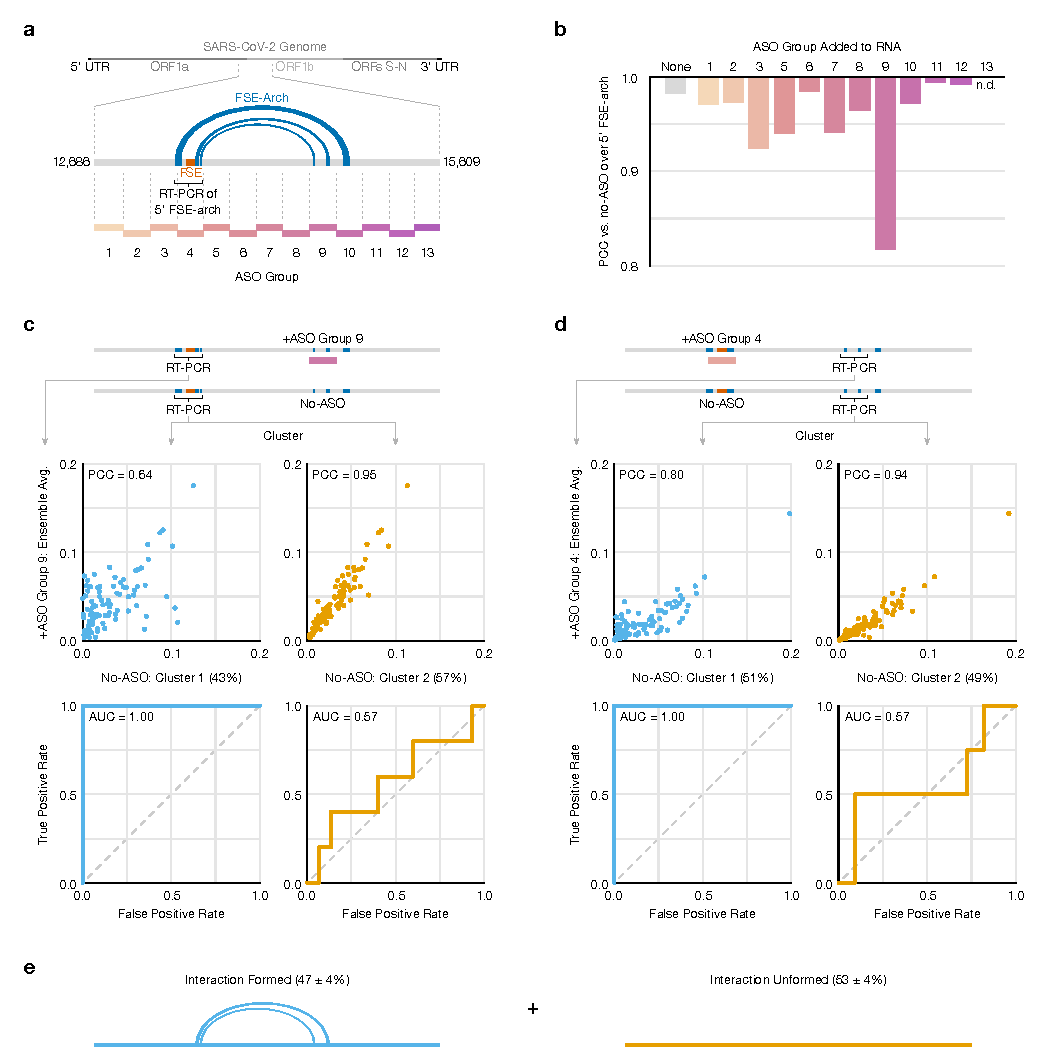
\includegraphics[width=\textwidth]{../MainFigures/sars2-tile/sars2-tile.pdf}
	\caption{}
	\label{tiles}
\end{figure}

\end{document}
